\section{Introduction}

\label{sec:intro}

An increased quality of living in a society often coincides with an increase in that society’s ability to freely gather and process data.  Distributed processing, also known as grid computing, offers a tool by which massive quantities of data can be processed at speeds tens of thousands of times faster than any centralized super computer.  This speed is directly proportional to the advancement of processing technology, currently progressing in accordance with Moore’s law. \\

At the same time, the Idle Processing Potential (IPP) which already exists in digital societies is severely underutilized.  From cell phones to personal computers to office workstations, the combined IPP of the world overshadows even the most robust decentralized super-computer, Bitcoin.
Gridcoin seeks to create a decentralized and sustainable distributed processing network which prioritizes both the utilization of IPP and the creation of a free to host ecosystem for researchers and individuals with data to process.
To accomplish this goal, Gridcoin has created a block-chain based digital asset which rewards individuals and entities which volunteer their IPP to the grid computing network, BOINC.  A single Gridcoin represents the value prescribed to a volunteered unit of IPP on the BOINC network.  The Gridcoin blockchain is secured through Proof of Stake.  Rewards are distributed through a protocol developed by Gridcoin called Distributed Proof of Research, or DPoR.\\

\begin{figure}
\centering
\includegraphics{figures/gridcoin-art-small}
\medskip
\caption{\textit{Gridcoin Art Medal depicting research in the fields of biology, electronics and astrophysics}}
\small
\end{figure}


BOINC, The Berkeley Open Infrastructure for Network Computing, is an open-source distributed processing network which provides scientists and enthusiasts with a means to host data for free. BOINC has been operating since 2002 and has and continues to process data that helps map the Milky Way, detect near earth asteroids, find prime numbers, fold proteins, test cures and vaccines, test chemical and molecular combinations, Search for Extraterrestrial Life (SETI), and more.\\

By directly rewarding those who volunteer their idle processing power to BOINC, Gridcoin creates an ecosystem in which valuable data, or a worthwhile project, is defined by an “open market of science” instead of a market of “pay-to-play”.  In other words, volunteers will move their IPP to projects which they deem of value with no need to consider the reward they will receive.\\

Although there are other configurations, a typical node runs both the BOINC client to download, execute and report results of scientific computations and the Gridcoin client. The gridcoin client performs several functions: like a bitcoin wallet it allows to transfer money from different addresses, it keeps the blockchain with transactions up to date talking to other nodes and verifying each new block for validity and tries to stake other blocks on the blockchain by collecting new transactions. The coinstake in the proposed new blocks for the own wallet corresponds to the amount of work done on BOINC expressed in gridcoins.\\

\subsection{BOINC}

BOINC is a system for distributing the workload of scientific simulations. Users of BOINC have a client running that solves work units (WU) for the specific projects. A work unit consists of code and specific parameters for which the code is run.  After the work unit is completed the BOINC client sends back the results to the BOINC servers, where the results are analyzed.\\

One example for a BOINC project is the World Community Grid [11], which consists of various other projects, for example to fight cancer or beat Ebola. SETI@home [20], which looks for signs of alien life by monitoring electromagnetic radiation from space for patterns, is another well-known project.  In total there are about 40 BOINC projects, but only the BOINC projects on the Whitelist help users earn Gridcoins. Each Gridcoin wallet can vote in polls about which projects can enter or exit the whitelist. New projects with interesting computational tasks enter it often and projects which do not have a constant supply of work units tend to be dropped by people's vote. \\

The information which researcher has computed how many work units is stored on the BOINC server. The unit of work done is a credit (cobblestone), which is 1,000 double-precision MFLOPS based on the Whetstone benchmark.  The Recently Averaged Credit (RAC) is the average amount of credits earned per day.\\

A CPID (Cross Project Identifier) is a number that links together the participation of a single user in all the different projects with a single common identifier, with a CPID one can see the research done by one user over all different projects this user participates in.\\

There are also teams in BOINC, users can join teams and the work done by each member of the team is added to get the work done by the team. It is necessary for a Gridcoin-researcher to be a part of team \textit{Gridcoin}, which on some projects is listed as \textit{gridcoin}, lowercase.

\begin{figure}
\centering
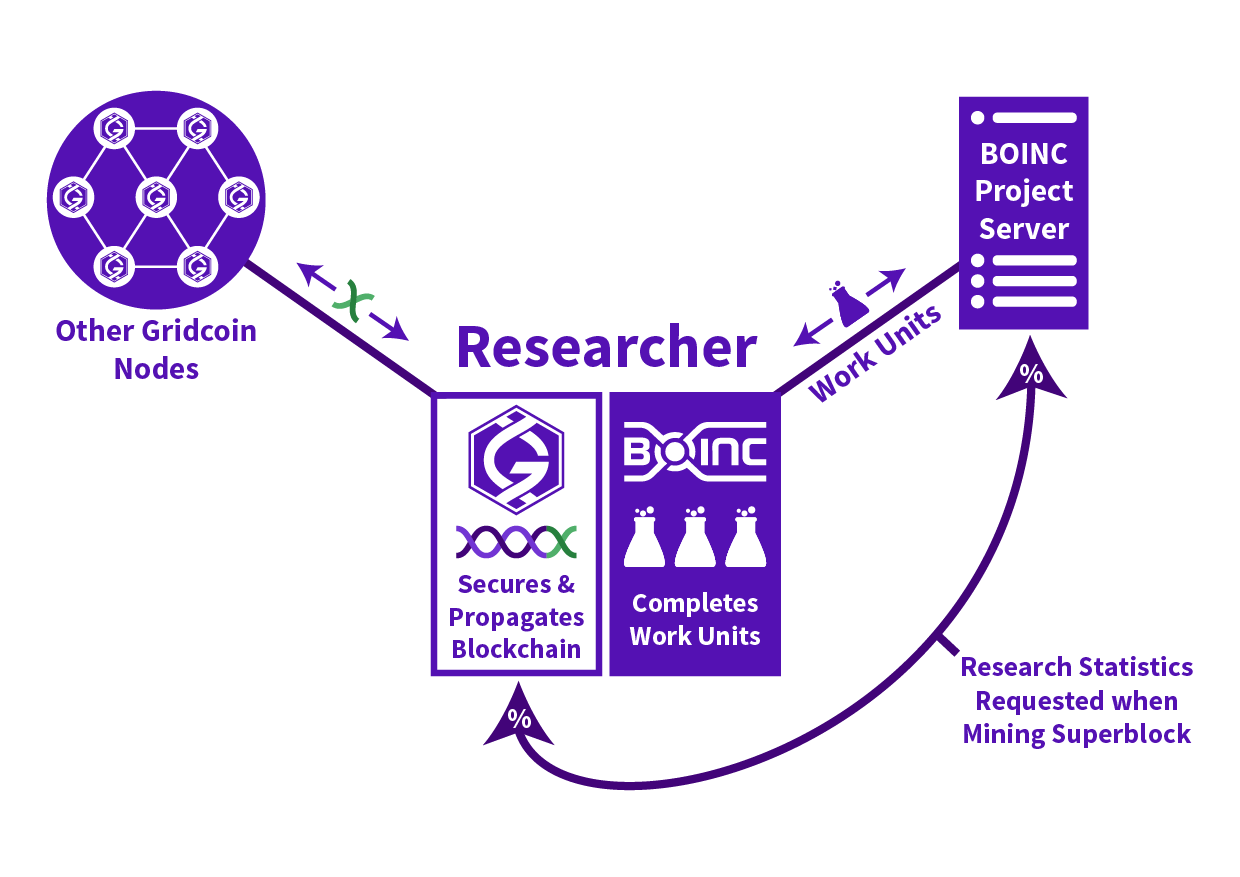
\includegraphics[scale=0.5]{figures/researcherdiagram_joshoeah}
\medskip
\caption{\textit{Gridcoin and BOINC Architecture} [5]}
\small
\end{figure}

\subsection{Gridcoin Client}

The Gridcoin Client is very similar to a Bitcoin client, inheriting substantial portions of source code from it. It is sometimes called a wallet, because it stores the Gridcoins owned by a user. The client allows to receive and send gridcoins to other clients. If it is attached to BOINC, it tries to mine blocks by collecting transactions and by showing that there was actual BOINC research done. From time to time, the client stakes gridcoins so that they earn an interest.

\subsection{Setting up a network node to earn Gridcoins}

To setup BOINC and the Gridcoin client to earn Gridcoins by running scientific simulations on your computer please follow the tutorials on www.gridcoin.us

The steps involved to become a solo miner are:
\begin{itemize}
  \item Install BOINC
  \item Add projects to BOINC that belong to the Whitelist [42]
  \item Install and configure Gridcoin wallet so that it is linked to BOINC 
  \item Acquire gridcoins by buying them on exchanges and move them to your wallet
  \item Send a beacon so that the wallet CPID is persisted in the blockchain
  \item Wait until client manages to stake first block with Proof of Stake and Proof of Research reward for your wallet.
\end{itemize}

On the mentioned website there are also instructions about mining in a common pool. There is also the possibility to be an investor by owning gridcoins and running the gridcoin client without being a BOINC researcher. In the latter case, the investor earns some interest on the gridcoins he owns, if he runs the wallet.\\

For exchanges that want to integrate Gridcoin in their infrastructure the client can be run entirely in textual mode out of a Linux bash shell. The daemon named \textit{gridcoinresearchd} implements the same commands with the same sintax as \textit{bitcoind}, making the integration of Gridcoin in the existing exchange infrastructure quick and harmless.\\
